% !TEX program = xelatex
\documentclass[12pt, a4paper]{article}
\input{packages.tex}
\input{settings.tex}

\begin{document}

% \maketitle
\begin{center}
    \LARGE \textbf{535521 Selected Topics in Visual Recognition using Deep Learning}\\[0.4em]
    \large Homework 4: Image Restoration\\
    \large HSU, PAO - HUA\\
    \normalsize NYCU AI System\\
    \vspace{0.5em}
    \normalsize \texttt{https://github.com/benhsu0828/NYCU_DLCV_Image_Restoration.git}
\end{center}

\vspace{1em}

\begingroup
\footnotesize
\section{Introduction}
\label{sec:intro}

This homework targets the image restoration track of NYCU DLCV HW4. The training set contains 3{,}200 paired (degraded, clean) images split evenly between two weather degradations -- 1{,}600 \textit{rain} and 1{,}600 \textit{snow} -- and the goal is to train a single all-in-one model that restores both without being told which degradation each test image suffers from. Submissions are scored by PSNR on a public leaderboard.

The assignment imposes three hard constraints: (i) no external data, (ii) no pretrained weights of any kind, and (iii) PromptIR~\cite{potlapalli2023promptir} must be used as the model. PromptIR is a natural fit because its \textit{PromptGenBlock} explicitly learns a set of degradation prototypes and lets the network condition itself on the input -- exactly the property we need for an all-in-one solution. Building strictly on this baseline, we add three groups of from-scratch modifications: \textbf{(a) architectural} (an AdaIR-style frequency-modulation branch, channel-attention inside every Transformer block, and gated prompt fusion in the decoder); \textbf{(b) optimization} (Charbonnier + SSIM + frequency losses, all implemented without any pretrained network); and \textbf{(c) training / inference hygiene} (weight EMA during training and an 8$\times$ geometric self-ensemble at test time).

\section{Method}
\label{sec:method}

Our baseline is the official PromptIR~\cite{potlapalli2023promptir}, which scores PSNR = 30.25 dB on the public leaderboard. To push beyond that, we make four targeted changes to the backbone and one change to the loss. Each change is implemented as an opt-in module so it can be ablated individually.

\subsection{Baseline: PromptIR}
PromptIR is built on a Restormer~\cite{zamir2022restormer}-style 4-level U-Net Transformer. Attention is computed along the channel dimension (Multi-Dconv Head Transposed Attention, MDTA), which makes high-resolution images tractable, and the feed-forward block uses a depthwise-conv gating (Gated-Dconv Feed-Forward Network, GDFN). The defining contribution of PromptIR is the \textbf{PromptGenBlock}: it maintains a small set of learnable ``degradation prototypes,'' produces input-dependent mixture weights from a global average pooling of the current feature map, and injects the weighted prompt back into three different decoder scales. This single design lets one network handle multiple degradation types without an explicit degradation label, which is exactly the property the all-in-one setting demands.

\subsection{Frequency Modulation Branch (AdaIR-style)}
Image restoration is closely tied to frequency content -- rain streaks, snow particles and motion blur all leave distinct signatures in the spectrum -- yet attention operates almost entirely in the spatial domain and is therefore weak at recovering high-frequency details. Inspired by AdaIR~\cite{cui2024adair} and FFTformer~\cite{kong2023fftformer}, we add a lightweight \texttt{FFTBlock} at the U-Net bottleneck. The block first transforms the feature into the frequency domain via 2D FFT, splits the spectrum into a low- and a high-frequency band with a learnable radial soft mask, modulates each band with channel-wise scaling ($\alpha_{low}, \alpha_{high}$) and a $1{\times}1$ conv, and finally inverse-FFTs and fuses the two bands with a $3{\times}3$ conv before adding a residual:
\begin{align}
M(r) &= \sigma\!\left(-\beta (r - \tau)\right), \quad r \in [0, 1] \text{ is the normalized distance from DC} \\
\mathrm{FFTBlock}(x) &= \mathrm{Conv}_{3\times3}\!\left([\alpha_l \cdot \mathrm{Conv}_l(\mathcal{F}^{-1}(\mathcal{F}(x) \cdot M)),\, \alpha_h \cdot \mathrm{Conv}_h(\mathcal{F}^{-1}(\mathcal{F}(x) \cdot (1-M)))]\right) + x
\end{align}
Both the cutoff $\tau$ and the sharpness $\beta$ are learnable scalars, so the network decides for itself where the low/high boundary should lie. We attach this block only at the latent because (i) the resolution is the lowest there so the FFT is cheap, and (ii) the latent feeds every decoder stage, giving the modulation its widest possible influence. The whole module is trained from scratch -- no pretrained spectral filter is used.

\subsection{Channel Attention (SE)}
PromptIR places no explicit importance on individual channels, yet in practice different channels carry different degradation patterns (rain streaks vs.\ snow particles vs.\ texture). We add a Squeeze-and-Excitation~\cite{hu2018se} module after the FFN of every \texttt{TransformerBlock}:
\begin{equation}
\mathrm{SE}(y) = y \odot \sigma\!\left(W_2\,\mathrm{GELU}(W_1\,\mathrm{GAP}(y))\right),
\end{equation}
with reduction ratio 8. The module is essentially two linear layers, so it adds negligible parameters and FLOPs while letting the network re-weight restoration-relevant channels adaptively.

\subsection{Gated Prompt Fusion}
The original PromptIR injects prompts into the decoder by concatenating the prompt to the image feature, passing the result through a TransformerBlock, and finally reducing the channel count with a $1{\times}1$ conv. This forced fusion can let prompt and image features interfere with each other. We replace it with a Gated-SCNN~\cite{takikawa2019gscnn}-style sigmoid gate that lets the network learn, position by position, how much to trust each source:
\begin{equation}
\mathrm{Fuse}(F, P) = g \odot W_f F + (1-g) \odot W_p P,\quad g = \sigma\!\left(W_g [F, P]\right),
\end{equation}
where $F$ is the image feature, $P$ is the prompt feature, and $W_f, W_p, W_g$ are all $1{\times}1$ convs.

\subsection{Loss Function}
The original training objective is pixel-wise L1, which is well known to encourage over-smooth outputs. We cannot use a VGG perceptual loss because the assignment forbids pretrained weights, so we adopt three fully from-scratch terms:
\begin{itemize}
    \item \textbf{Charbonnier loss}~\cite{charbonnier1994two}: $\mathcal{L}_{\text{char}} = \sqrt{(\hat{y}-y)^2 + \epsilon^2}$, a smooth L1 variant that is more robust to outliers.
    \item \textbf{SSIM loss}~\cite{wang2004ssim}: $\mathcal{L}_{\text{ssim}} = 1 - \mathrm{SSIM}(\hat{y}, y)$, computed with an $11{\times}11$ Gaussian window implemented in-house; this captures structural similarity that pixel losses ignore.
    \item \textbf{Frequency loss}: $\mathcal{L}_{\text{freq}} = \|\mathcal{F}(\hat{y}) - \mathcal{F}(y)\|_1$ (real + imag components concatenated), aligning prediction and target in the frequency domain so that high-frequency details are penalized directly.
\end{itemize}
The total loss is
\begin{equation}
\mathcal{L}_{\text{total}} = \mathcal{L}_{\text{char}} + \lambda_{\text{ssim}}\,\mathcal{L}_{\text{ssim}} + \lambda_{\text{freq}}\,\mathcal{L}_{\text{freq}},
\end{equation}
with $\lambda_{\text{ssim}} = 0.2$ and $\lambda_{\text{freq}} = 0.05$. None of the terms depends on a pretrained network, so the resulting model is fully rule-compliant.

\subsection{Weight EMA (Exponential Moving Average)}
Following the weight-averaging idea behind Mean Teacher~\cite{tarvainen2017meanteacher}, we maintain an exponentially-averaged shadow copy of the model weights during training:
\begin{equation}
\theta_{\text{EMA}}^{(t)} = \alpha \cdot \theta_{\text{EMA}}^{(t-1)} + (1-\alpha) \cdot \theta^{(t)},\quad \alpha = 0.999.
\end{equation}
The EMA weights are used both for validation and for the final inference. Intuitively, averaging smooths out the late-training oscillations that pure SGD-style updates leave behind and tends to land in a flatter local minimum than the raw weights.

\subsection{Test-Time Augmentation (x8 Self-Ensemble)}
At inference time we apply 8 information-preserving geometric transforms (identity / horizontal flip / vertical flip / horizontal+vertical flip / rot90 / rot180 / rot270 / transpose), run a forward pass for each, invert the transform on the output, and average the eight predictions:
\begin{equation}
\hat{y}_{\text{TTA}} = \frac{1}{8} \sum_{i=1}^{8} T_i^{-1}\!\left(f_\theta(T_i(x))\right).
\end{equation}
This is a standard trick in image restoration~\cite{lim2017edsr}: it adds no parameters and costs only $8\times$ inference compute, leaving training untouched.

\subsection{Overall Pipeline}
The new modules are not chained into a single sequential block. They are \textbf{injected at different points} inside the PromptIR backbone:
\begin{itemize}
    \item SE is plugged into every \texttt{TransformerBlock} after the FFN.
    \item The AdaIR-style FFTBlock is attached in parallel at the latent.
    \item Gated fusion replaces the prompt-concat fusion at all three decoder scales.
    \item Charbonnier + SSIM + frequency losses replace the original pure L1.
    \item Weight EMA is updated during training.
    \item $8\times$ self-ensemble TTA is applied at inference.
\end{itemize}
All modules can be toggled independently via CLI flags, so each one can be ablated cleanly. Crucially, every addition is trained from scratch and uses only the provided dataset, so the system complies with the assignment rules.

\subsection{Data Processing and Augmentation}
The provided training set contains 3{,}200 paired images (1{,}600 rain + 1{,}600 snow). We hold out the last 100 indices of each type as a validation split, giving 3{,}000 train / 200 val pairs. During training every sample is randomly cropped to $128{\times}128$, then independently horizontally flipped (p = 0.5), vertically flipped (p = 0.5), and rotated by $k{\cdot}90^{\circ}$ with $k$ uniformly sampled from $\{0, 1, 2, 3\}$. No external data, no pretrained augmentation policies, no GAN-generated samples.

\subsection{Hyperparameters}
\label{sec:hparam}
All hyperparameters are listed in Table~\ref{tab:hparam}. We use AdamW with a cosine schedule and a small weight decay. Loss weights were chosen so that no single auxiliary term dominates the Charbonnier term.

\begin{table}[H]
    \centering
    \small
    \begin{tabular}{ll}
        \toprule
        \textbf{Hyperparameter} & \textbf{Value} \\
        \midrule
        Optimizer & AdamW ($\beta_1{=}0.9$, $\beta_2{=}0.999$) \\
        Weight decay & $1{\times}10^{-4}$ \\
        Initial learning rate & $2{\times}10^{-4}$ \\
        LR schedule & CosineAnnealingLR ($T_{\max}{=}\text{epochs}$, $\eta_{\min}{=}1{\times}10^{-6}$) \\
        Epochs & 150 \\
        Batch size & 8 \\
        Patch size (random crop) & $128{\times}128$ \\
        Augmentation & h-flip (p=0.5), v-flip (p=0.5), rot90 $\times \{0,1,2,3\}$ \\
        Loss weights & $\lambda_{\text{ssim}}=0.2$, $\lambda_{\text{freq}}=0.05$ \\
        SE reduction ratio & 8 \\
        EMA decay $\alpha$ & 0.999 \\
        Test-time augmentation & $8\times$ self-ensemble \\
        Random seed & 42 \\
        \bottomrule
    \end{tabular}
    \caption{Training hyperparameters.}
    \label{tab:hparam}
\end{table}

\section{Results}
\label{sec:results}

\subsection{Leaderboard}
Table~\ref{tab:leaderboard} compares the original PromptIR with our final modified model on the public leaderboard. The full set of modifications lifts the public PSNR from 30.25 dB to 31.07 dB.

\begin{table}[H]
    \centering
    \small
    \begin{tabular}{lc}
        \toprule
        \textbf{Submission} & \textbf{Public PSNR (dB)} \\
        \midrule
        \texttt{pred\_baseline.zip} (vanilla PromptIR) & 30.25 \\
        \texttt{pred\_round2.zip} (ours, full pipeline) & \textbf{31.07} \\
        \midrule
        $\Delta$ over baseline & $+0.82$ \\
        \bottomrule
    \end{tabular}
    \caption{Public leaderboard PSNR. ``Ours'' includes the AdaIR-style FFTBlock, SE, gated prompt fusion, Charbonnier + SSIM + frequency losses, weight EMA and $8\times$ self-ensemble TTA.}
    \label{tab:leaderboard}
\end{table}

\subsection{Competition Ranking}
Figure~\ref{fig:competition} shows our standing on the public leaderboard.

\begin{figure}[H]
    \centering
    
\includegraphics[width=0.9\linewidth]{figure/competition.png}
    \caption{Public-leaderboard ranking for the final submission.}
    \label{fig:competition}
\end{figure}

\subsection{Wandb Logs}
Figure~\ref{fig:wandb_curves} plots the training loss and the EMA-evaluated validation PSNR. The loss decreases monotonically under the cosine schedule and the validation PSNR rises steadily, with no obvious sign of overfitting up to 150 epochs.

\begin{figure}[H]
    \centering
    \begin{subfigure}[t]{0.48\linewidth}
        \centering
        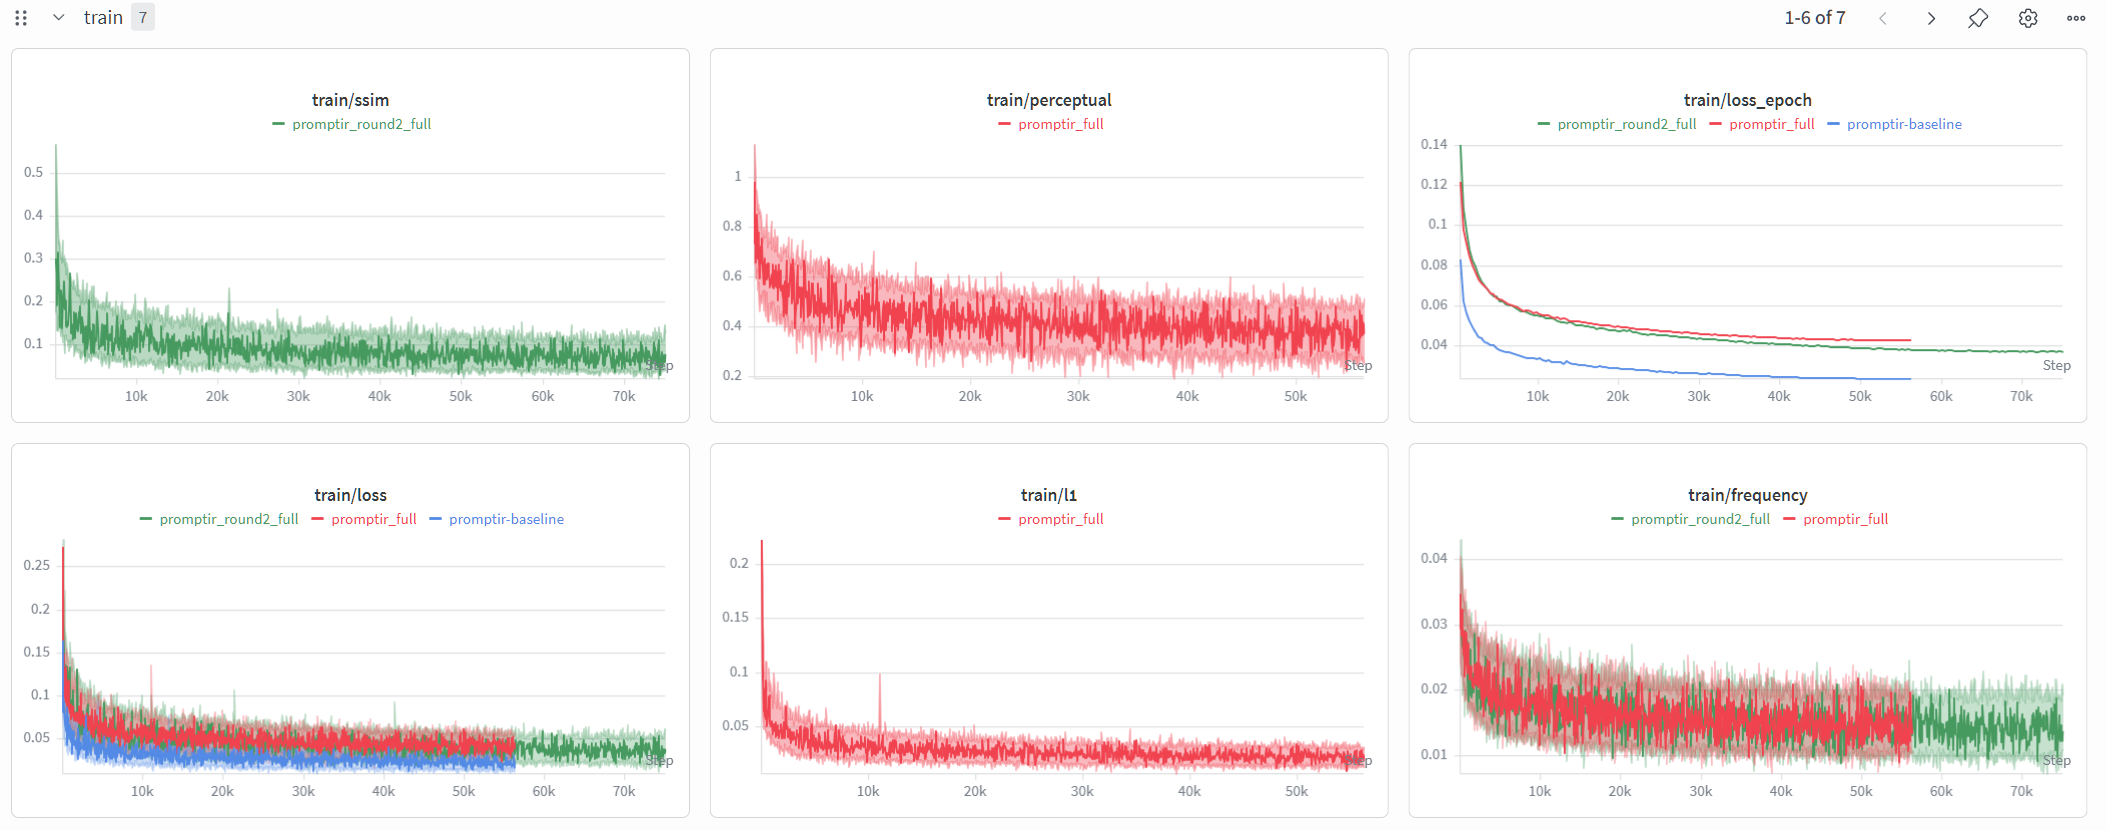
\includegraphics[width=\linewidth]{figure/training_loss.png}
        \caption{Training loss curve.}
        \label{fig:train_loss}
    \end{subfigure}
    \hfill
    \begin{subfigure}[t]{0.48\linewidth}
        \centering
        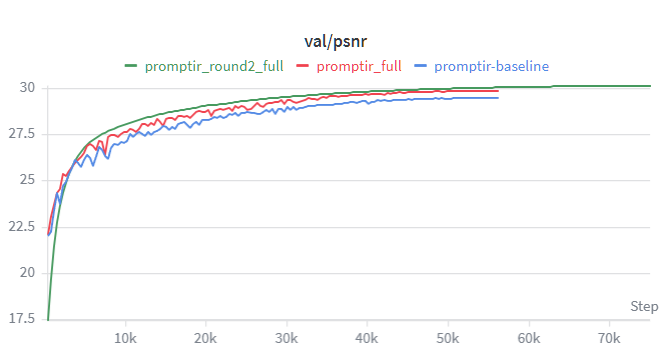
\includegraphics[width=\linewidth]{figure/val_result.png}
        \caption{Validation PSNR curve (EMA weights).}
        \label{fig:val_psnr}
    \end{subfigure}
    \caption{Training logs: (a) training loss, (b) validation PSNR.}
    \label{fig:wandb_curves}
\end{figure}

\subsection{Qualitative Results}
Figure~\ref{fig:val_example} shows representative qualitative results on the validation split. The model removes rain streaks and snow particles while keeping edges and texture sharp.

\begin{figure}[H]
    \centering
    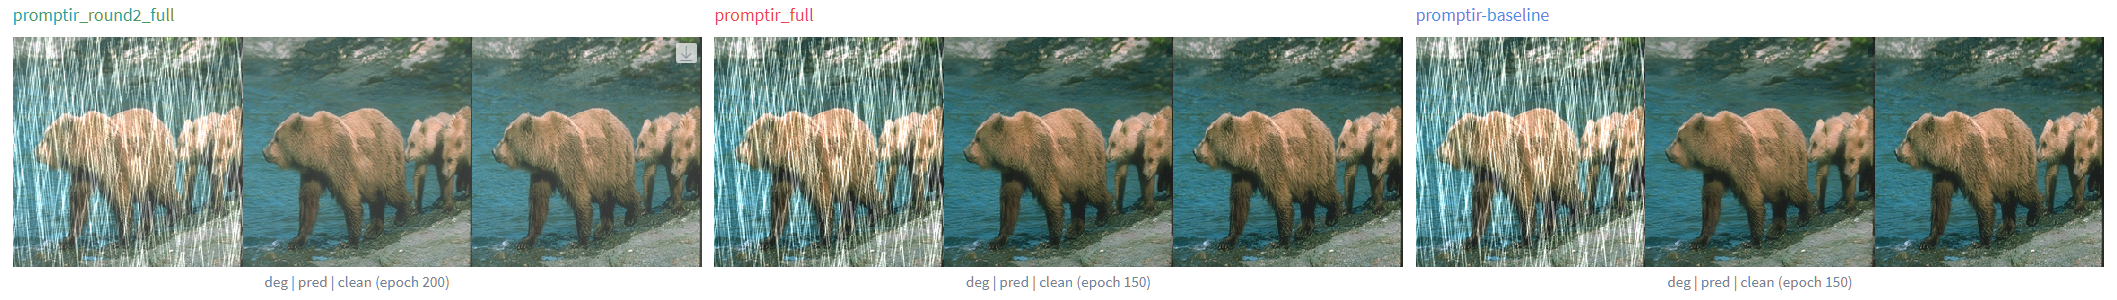
\includegraphics[width=0.95\linewidth]{figure/val_example.png}
    \caption{Qualitative results on the validation split. Left: degraded input; middle: model prediction; right: clean ground truth.}
    \label{fig:val_example}
\end{figure}



\bibliographystyle{unsrt}
\bibliography{references}
\endgroup


\end{document}
